%% This LaTeX-file was created by <amundson> Tue Dec 14 12:28:59 1999
%% LyX 0.12 (C) 1995-1998 by Matthias Ettrich and the LyX Team

%% Do not edit this file unless you know what you are doing.
\documentclass[12pt,english]{article}
\usepackage[T1]{fontenc}
\usepackage{times}
\usepackage{babel}
\usepackage{graphics} \usepackage{epsfig}

\makeatletter


%%%%%%%%%%%%%%%%%%%%%%%%%%%%%% LyX specific LaTeX commands.
\newcommand{\LyX}{L\kern-.1667em\lower.25em\hbox{Y}\kern-.125emX\spacefactor1000}

%%%%%%%%%%%%%%%%%%%%%%%%%%%%%% Textclass specific LaTeX commands.
\newenvironment{lyxcode}
  {\begin{list}{}{
    \setlength{\rightmargin}{\leftmargin}
    \raggedright
    \setlength{\itemsep}{0pt}
    \setlength{\parsep}{0pt}
    \ttfamily}%
   \item[]}
  {\end{list}}

%%%%%%%%%%%%%%%%%%%%%%%%%%%%%% User specified LaTeX commands.
\date{Manual Version 1.02\\December 14, 1999}
\makeatother

\begin{document}


\title{SoftRelTools Manual}


\author{James Amundson \\
Computing Division\\
Fermi National Accelerator Laboratory }

\maketitle
\newpage

\tableofcontents

\newpage


\section*{About this manual}

This manual describes SoftRelTools version 2. It is intended to augment the
documentation in ``A UNIX Based Software Management System,'' edited by Robert
Harris, Computing Division Note: GU0013, which provides a more general introduction
to SoftRelTools. It is available at 

\begin{lyxcode}
<http://www-cdf.fnal.gov/offline/code\_management/run2\_cmgt/run2\_cmgt.html>.
\end{lyxcode}

\subsection*{Manual Changelog}

\begin{description}
\item [v1.01]April 28, 1999: Inital public version.
\item [v1.02]December 14, 1999: Updated name of cvs repository.
\end{description}

\section{Introduction}

The primary purpose of SoftRelTools version 2 is to provide a backward-compatible
replacement for the original SoftRelTools written by Bob Jacobsen. SoftRelTools
is designed to be easier to use and to maintain than the original SoftRelTools.
Ease of use and maintainability are enhanced by increased functionality and
modular structure. Maintainability is further enhanced by the seperation of
the basic tool from project and site specific settings through an inheritance
heierarchy.

The modules and their relationships are described by the following figure:

\vspace{0.3cm}
{\centering \resizebox*{0.75\columnwidth}{!}{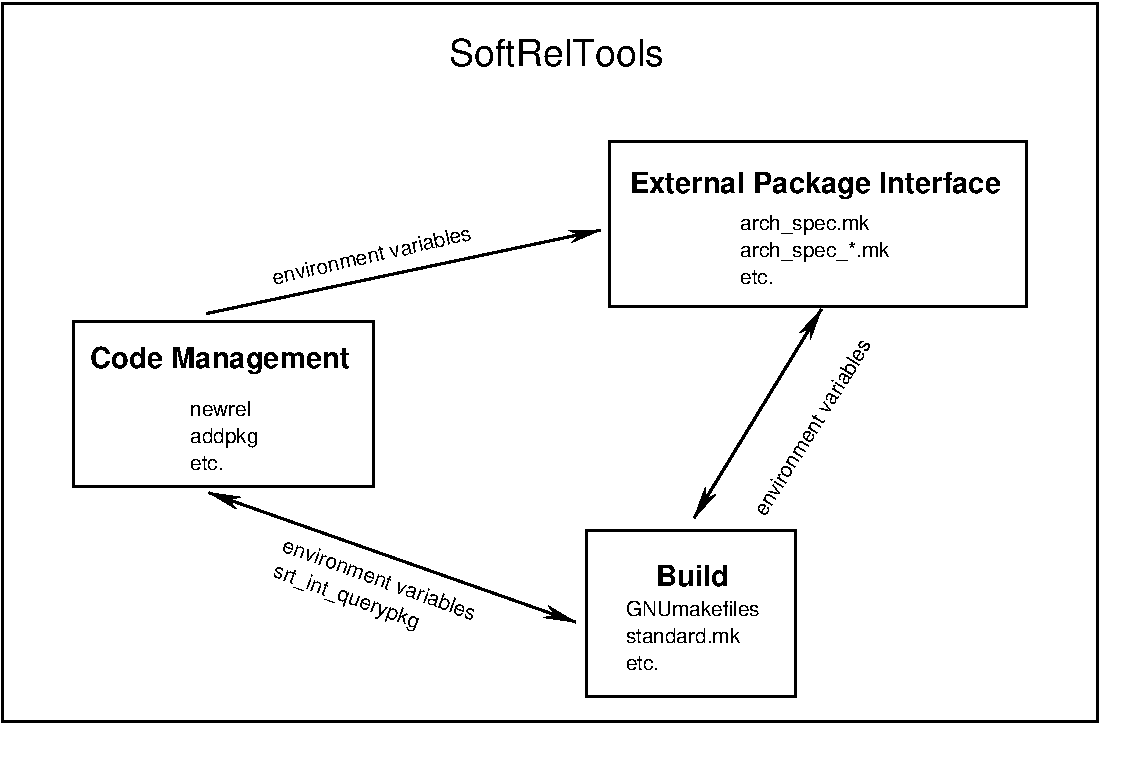
\epsfig{file=modules.eps,clip=}} \par}
\vspace{0.3cm}

The inheritance heierarchy from base to project and site-specific settings is
orthogonal to the separation of the tool into modules. In the figure below,
each pane represents the collection of modules shown in the figure above.

\vspace{0.3cm}
{\centering \resizebox*{0.75\columnwidth}{!}{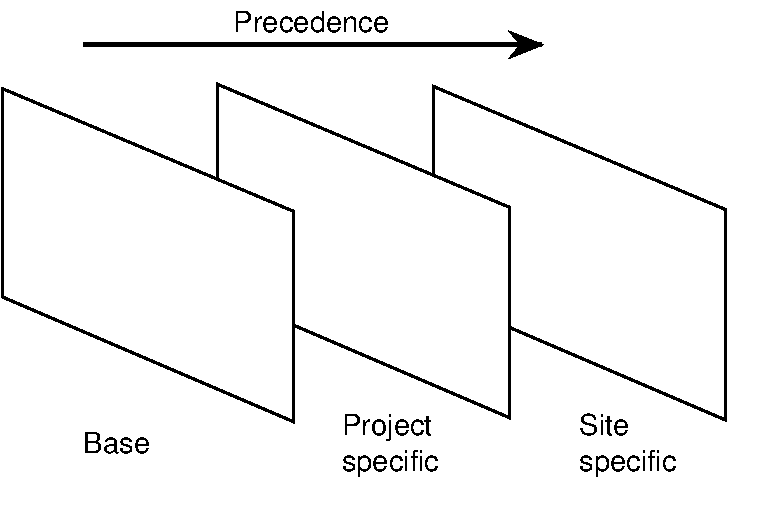
\epsfig{file=inheritance.eps,clip=}} \par}
\vspace{0.3cm}

The SoftRelTools base is largely self-contained. The project and site specific
behavior is implemented through optional additional packages, SRT\_\$PROJECT
and SRT\_SITE.


\section{SoftRelTools for users}


\subsection{Introduction}

All of the publicly available SoftRelTools files live in a distribution directory.
For the purposes of the manual we we refer to this directory as \$SRT\_DIST.
In order to use SoftRelTools, users must have sourced the file \$SRT\_DIST/srt/srt.csh
or \$SRT\_DIST/srt/srt.sh, depending on the users' shell. Of course, this assumes
that a SoftRelTools distribution in \$SRT\_DIST has been installed. (See SoftRelTools
for librarians.) After srt.(c)sh has been sourced, the command ``srt\_setup''
will set up SoftRelTools for use. srt\_setup is described in the srt\_setup
man page and in the section on the SoftRelTools environment.

The following example shows how a user can work with a package ``Hello'' that
is part of a release ``development''. It assumes that SRT has been set up.

\begin{enumerate}
\item Create a test release called ``myrelease''

\begin{lyxcode}
newrel~-{}-test~development~myrelease

cd~myrelease
\end{lyxcode}
\item Add the Hello package to ``myrelease''

\begin{lyxcode}
addpkg~Hello
\end{lyxcode}
\item Set the local context, i.e., tell SRT to work with the current release. This
is optional, but it speeds compilation.

\begin{lyxcode}
srt\_setup~-a
\end{lyxcode}
\item Build all packages in the release

\begin{lyxcode}
gmake
\end{lyxcode}
\item Here is a transcript of the steps above on my machine:
\end{enumerate}
\begin{lyxcode}
{\footnotesize >~newrel~-{}-test~development~myrelease}{\footnotesize \par}

{\footnotesize read~user~srtrc}{\footnotesize \par}

{\footnotesize Creating~a~test~release~\char`\"{}myrelease\char`\"{}~in~the~directory}{\footnotesize \par}

{\footnotesize ~~~~/home/amundson/work}{\footnotesize \par}

{\footnotesize Linking~tmp~to~/tmp/myrelease/tmp}{\footnotesize \par}

{\footnotesize Linking~bin~to~/tmp/myrelease/bin}{\footnotesize \par}

{\footnotesize Linking~lib~to~/tmp/myrelease/lib}{\footnotesize \par}

{\footnotesize >~cd~myrelease/}{\footnotesize \par}

{\footnotesize >~addpkg~Hello}{\footnotesize \par}

{\footnotesize Release~development~uses~Hello~version~HEAD,~will~check~that~out}{\footnotesize \par}

{\footnotesize Adding~package~\char`\"{}Hello\char`\"{}~to~\char`\"{}.\char`\"{}.}{\footnotesize \par}

{\footnotesize cvs~checkout:~Updating~Hello}{\footnotesize \par}

{\footnotesize U~Hello/GNUmakefile}{\footnotesize \par}

{\footnotesize U~Hello/Hello.cc}{\footnotesize \par}

{\footnotesize U~Hello/Hello.h}{\footnotesize \par}

{\footnotesize U~Hello/HelloExample.cc}{\footnotesize \par}

{\footnotesize >~srt\_setup~-a}{\footnotesize \par}

{\footnotesize >~gmake}{\footnotesize \par}

{\footnotesize <{*}{*}include{*}{*}>}{\footnotesize \par}

{\footnotesize <{*}{*}include{*}{*}>~Hello}{\footnotesize \par}

{\footnotesize <{*}{*}lib{*}{*}>}{\footnotesize \par}

{\footnotesize <{*}{*}lib{*}{*}>~Hello}{\footnotesize \par}

{\footnotesize <{*}{*}compiling{*}{*}>~Hello.cc}{\footnotesize \par}

{\footnotesize <{*}{*}building~library{*}{*}>~libHello}{\footnotesize \par}

{\footnotesize <{*}{*}bin{*}{*}>}{\footnotesize \par}

{\footnotesize <{*}{*}bin{*}{*}>~Hello}{\footnotesize \par}

{\footnotesize <{*}{*}compiling{*}{*}>~HelloExample.cc}{\footnotesize \par}

{\footnotesize <{*}{*}building{*}{*}>~HelloExample}{\footnotesize \par}

{\footnotesize >}{\footnotesize \par}
\end{lyxcode}
The lines ``read user srtrc'' and ``Linking... to ...'' after newrel are
a result of my \~{}/.srtrc file. See the section on user preferences for the
code management system.


\subsection{Details}

To learn more about the commands newrel, addpkg, etc., read the section on the
code management system. To learn more about building your own packages, read
the section on the build system.


\section{SoftRelTools for librarians}


\subsection{Installing SoftRelTools}

(The following information is duplicated in the file README.install in the SoftRelTools/install
directory.)

This version of SoftRelTools needs two things to get started:

\begin{enumerate}
\item A working boot release. 
\item A properly installed srt directory in the main release area.
\end{enumerate}
Once these two things are in place, users must

\begin{enumerate}
\item Source the \$SRT\_DIST/srt/srt.(c)sh file appropriate for their shells. 
\item Execute \char`\"{}srt\_setup\char`\"{}.
\end{enumerate}
Instructions for creating the boot release and srt directory follow:


\subsubsection*{To create a completely new SoftRelTools distribution:}

\begin{enumerate}
\item Get srt\_distribution.tar and untar it. (srt\_distribution.tar is distributed
separately.) 
\item You now have a directory called srt\_distribution. Move/rename it to whatever
you want, but the instructions will refer to this directory as srt\_distribution.
\item cd to srt\_distribution/srt directory.
\item Execute the install script with \char`\"{}./install -p <your project>\char`\"{}.
You can see the options to install with \char`\"{}./install --help\char`\"{}.
The install script writes the location of the srt directory to the srt.(c)sh
files. If you move the distribution, you will have to run install again. The
project and cvsroot files can be modified by hand if you wish.
\end{enumerate}

\subsubsection*{To update an old SoftRelTools distribution to work with the new SoftRelTools:}

\begin{enumerate}
\item Untar the file boot\_release.tar from this directory in your distribution \char`\"{}releases\char`\"{}
directory.
\item Copy the srt directory from this directory to the distribution directory (the
directory the old SoftRelTools called \$BFDIST.)
\item cd to the new srt directory
\item See step 4above.
\end{enumerate}

\subsection{Setting project preferences}

There are several new files that can hold settings that apply to all users.

\begin{description}
\item [\$SRT\_DIST/srt/cvsroot]holds the default value of CVSROOT for the distribution.
It can be overridden for each package; see below. The contents of this file
can be set by the install script or by hand.
\item [\$SRT\_DIST/srt/project]holds the name of the project. It corresponds to the
EXPERIMENT variable in the old SRT. There can be only one project per distribution.
The contents of this file can be set by the install script or by hand.
\item [\$SRT\_DIST/srt/srt.csh]is the file to be sources by csh and tcsh users. Only
one line of it should ever be modified. The install script modifies it for you.
\item [\$SRT\_DIST/srt/srt.sh]the file to be sources by ksh, zsh and bash users. Only
one line of it should ever be modified. The install script modifies it for you.
\item [\$SRT\_DIST/srt/srt\_envrc]contains default environment variable settings.
See the section on environment variables.
\item [\$SRT\_DIST/srt/srtrc]contains default system settings for directory creation/linking
in newrel. See the section on code management.
\item [\$SRT\_DIST/packages/<package>/cvsroot]is an optional file for each package.
If it exists, addpkg will automatically use it to determine the value of CVSROOT
for <package>. This file will be written automatically if newpkg is called with
the -d <cvsroot> argument. It can also me modified by hand.
\end{description}

\subsection{The project-specific package}

SoftRelTools will look for the package SRT\_\$SRT\_PROJECT (i.e., SRT\_D0, SRT\_CDF,
etc.). This package can be used to augment and/or replace behavior of the central
SoftRelTools. The mechanism for this is described in the section on the inheritance
hierarchy.


\subsection{The site-specific package}

The package SRT\_SITE (note the fixed name) is similar to the project-specific
package. It is only intended for situations where two different machines for
the same project need to behave differently. Its behavior supersedes both the
default behavior and the project-specific behavior.


\section{The inheritance hierarchy}


\subsection{Introduction}

The version of SoftRelTools at Fermilab is modified frequently -- on the order
of once per day. These changes fall into two categories: 1) Bug fixes. 2) Local
changes in settings, etc. The goal of the inheritance hierarchy in SoftRelTools
is to allow projects to be able to make both kinds of changes quickly, without
having to worry about affecting other projects. Changes of the first type can
be incorporated into the base package in a controlled manner. Changes of the
second type can stay with the projects, where they belong.

As the term implies, the inheritance hierarchy is based on the concepts of object-oriented
design. Think of the site-specific parts of SoftRelTools inheriting from the
project-specific parts, which inherit from the base. However, SoftRelTools is
implemented in primarily in GNU Make and Bourne Shell -- neither of which are
very well-suited to object-oriented programming. ``Inheritance'' in SoftRelTools
should really be considered an analogy. The analogy will break down if pushed
too far.

All of the modules in SoftRelTools can be modified first at the project level
then the site level. The site has the final word. There are two mechanisms available:

\begin{enumerate}
\item All the modules of SoftRelTools look in the ``special'' subdirectory of the
project and site packages. If a file corresponding to the current file exists
in the ``special'' directory it is sourced. The specialization files are included
in addition to the original file, the purpose being to augment or modify the
behavior of the base package. This is the preferred method of incorporating
changes.
\item The include paths in SoftRelTools also look in the project and site packages.
This allows replacement of the SoftRelTools base files. The replacement method
should only be used if the override method is unsuitable. It is considered a
goal that replacement does not need to be used. Replacement files go in the
``SoftRelTools'' subdirectory of the project and site packages.
\end{enumerate}

\subsection{Details}


\subsubsection{Makefile fragments}

All makefile fragments in SoftRelTools/include look for the a corresponding
file in SRT\_\$SRT\_PROJECT/special. Files in subdirectories of SoftRelTools/include
go into the corresponding subdirectories of SRT\_\$SRT\_PROJECT/special. A few
special files can be specialized both at the beginning and the end:

\begin{description}
\item [standard.mk]looks for pre\_standard.mk and post\_standard.mk.
\item [GNUmakefile.main]looks for pre\_GNUmakefile.main and post\_GNUmakefile.main.
\end{description}
All other files look for files of the same name as themselves.


\subsubsection{Scripts}

All of the scripts in SoftRelTools consist of a set of subroutines, including
one called ``main''. If specialization files are found in the ``scripts''
subdirectory of the project-specific package, they are sourced before any of
the subroutines are called. The specialization files can contain replacements
for old subroutines and/or new subroutines.


\subsubsection{Examples}

\begin{itemize}
\item Add a new target to standard.mk

\begin{itemize}
\item put the lines
\end{itemize}
\begin{lyxcode}
foo:

~~~~echo~``bar''
\end{lyxcode}
in special/post\_standard.mk in the project-specific package. Now ``gmake foo''
will return ``bar''.

\item Add the --no\_exceptions flag to the C++ compiler flags for the Kai compiler:

\begin{itemize}
\item put the line
\end{itemize}
\begin{lyxcode}
override~CXXFLAGS~+=~-{}-no\_exceptions~
\end{lyxcode}
in the special/compilers/KCC.mk in the project-specific package.

\item Provide additional actions for addpkg

\begin{itemize}
\item put the lines
\end{itemize}
\begin{lyxcode}
extra\_actions~()~\{

~~~~~~~~echo~\char`\"{}Now~executing~top~secret~extra~actions\char`\"{}

\}

~

main~()~\{

~~~~~~~script\_defaults

~~~~~~~process\_args~\${*}

~~~~~~~actions

~~~~~~~ods\_actions

\}
\end{lyxcode}
in scripts/addpkg in the project-specific package. Now addpkg will print an
extra message every time it is called. Notice that this example required both
providing a new subroutine, extra\_actions, and a replacing an existing routine,
main.

\end{itemize}

\section{The environment variables}


\subsection{srt\_setup and srt\_environment}

SoftRelTools includes two commands, srt\_setup and srt\_environment, for examining
and manipulating the user environmental variables. The former is actually an
alias that calls the latter with certain options. The default behavior for srt\_environment
is to print the current settings. Sample output is below.

\begin{lyxcode}
{\footnotesize SRT~settings:}{\footnotesize \par}

{\footnotesize Variables~for~backward~compatibility:}{\footnotesize \par}

{\footnotesize BFARCH~=~Linux2-KCC\_3\_3}{\footnotesize \par}

{\footnotesize BFDIST~=~/home/amundson/work/dist}{\footnotesize \par}

{\footnotesize BFCURRENT~=~development}{\footnotesize \par}

{\footnotesize ~}{\footnotesize \par}

{\footnotesize Automatic~and~derived~variables:}{\footnotesize \par}

{\footnotesize PATH~=~/home/amundson/work/myrelease/bin/Linux2-KCC\_3\_3:/home/amundson/work/dist}{\footnotesize \par}

{\footnotesize /releases/development/bin/Linux2-KCC\_3\_3:/fnal/ups/prd/kai/v3\_3f\_1/Linux+2/KCC\_B}{\footnotesize \par}

{\footnotesize ASE/bin:/home/amundson/work/dist/releases/boot/bin/generic:/opt/kde/bin:/fnal/up}{\footnotesize \par}

{\footnotesize s/prd/ups/v4\_3/Linux+2/bin:/opt/kde/bin:/home/amundson/work/dist/releases/boot/b}{\footnotesize \par}

{\footnotesize in/generic:/home/amundson/bin:/usr/sbin:/bin:/usr/bin:/etc:/usr/etc:/usr/bin/X11}{\footnotesize \par}

{\footnotesize :/usr/local/bin:.:/home/t1/amundson/bin:/home/t1/amundson/bin}{\footnotesize \par}

{\footnotesize LD\_LIBRARY\_PATH~=~/home/amundson/work/myrelease/lib/Linux2-KCC\_3\_3:/home/amundso}{\footnotesize \par}

{\footnotesize n/work/dist/releases/development/lib/Linux2-KCC\_3\_3:}{\footnotesize \par}

{\footnotesize SRT\_PRIVATE\_CONTEXT~=~/home/amundson/work/myrelease}{\footnotesize \par}

{\footnotesize SRT\_PUBLIC\_CONTEXT~=~/home/amundson/work/dist/releases/development}{\footnotesize \par}

{\footnotesize MAKEFILES~=~\char`\"{}SoftRelTools/preamble.mk\char`\"{}}{\footnotesize \par}

{\footnotesize MAKEFLAGS~=~\char`\"{}-r~-I/home/amundson/work/myrelease/SRT\_ODS~-I/home/amundson/work/di}{\footnotesize \par}

{\footnotesize st/releases/development/SRT\_ODS~-I/home/amundson/work/myrelease/include~-I/home/}{\footnotesize \par}

{\footnotesize amundson/work/dist/releases/development/include\char`\"{}}{\footnotesize \par}

{\footnotesize CVSROOT~=~/home/amundson/repository}{\footnotesize \par}

{\footnotesize SRT\_SUBDIR~=~Linux2-KCC\_3\_3}{\footnotesize \par}

{\footnotesize SRT\_PROJECT~=~ODS}{\footnotesize \par}

{\footnotesize SRT\_ARCH~=~Linux2}{\footnotesize \par}

{\footnotesize SRT\_ENV\_SET~=~yes}{\footnotesize \par}

{\footnotesize ~}{\footnotesize \par}

{\footnotesize User~settable~variables:}{\footnotesize \par}

{\footnotesize SRT\_LOCAL~=~/home/amundson/work/myrelease}{\footnotesize \par}

{\footnotesize SRT\_DIST~=~/home/amundson/work/dist}{\footnotesize \par}

{\footnotesize SRT\_BASE\_RELEASE~=~development}{\footnotesize \par}

{\footnotesize SRT\_CXX~=~KCC\_3\_3}{\footnotesize \par}

{\footnotesize SRT\_QUAL~=~default}{\footnotesize \par}
\end{lyxcode}
The most important changes from the original SoftRelTools settings are the replacement
of SRT\_ for BF as the variable prefix and the splitting of the BFARCH architecture-C++
compiler combination into SRT\_ARCH and SRT\_CPP, respectively. SoftRelTools
currently maintains the appropriate values of the BF variables, but it does
not use them internally

The first time srt\_setup is called, variables are set to their default settings,
SRT\_CXX=\$DEFAULT\_SRT\_CXX, etc. The defaults can be restored later by ``srt\_setup
-d''.

Users can alter the values of variables by putting one or more assignments on
the command line

\begin{lyxcode}
srt\_setup~SRT\_CXX=EGCS\_1\_1

srt\_setup~SRT\_QUAL=maxopt~SRT\_BASE\_RELEASE=test
\end{lyxcode}

\subsection{System defaults}

srt\_setup and srt\_environment source the file \$SRT\_DIST/srt/srt\_envrc.
This allows the librarian to set defaults for an entire project. For example,
the srt\_envrc might contain the lines

DEFAULT\_SRT\_CXX=KCC\_3\_3

DEFAULT\_SRT\_BASE\_RELEASE=development

Since the file is sourced by the shell script, it can contain any shell commands.
Only the resulting value of the variables matter.


\subsection{User defaults}

srt\_setup and srt\_environment also source the file \$HOME/.srt\_envrc. (Note
the presence of a leading dot in the user file, but not in the system file.)
This allows the user to set his/her own defaults. Again, the file is sourced
by the shell script, so it can contain any shell commands.


\section{The code management system}


\subsection{Introduction}

The scripts for the code management system are described by the man pages. Additionally,
every script will describe its own actions and options when invoked with ``--help''
or an argument it does not understand. The ``newrel'' command looks for system
and user preferences. 

Scripts with the prefix ``srt\_int'' are used internally by SoftRelTools.
They will not generally be useful to users. Note that the srt\_int\_querypkg
script is technically part of the build system, not the code management system.
That means that changes to the build system can affect srt\_int\_querypkg. The
code management scripts are designed to be independent of the build system.


\subsection{System preferences for newrel}

newrel sources the file \$SRT\_DIST/srt/srtrc for directory creation preferences.
If the variable ``extra\_dirs'' is defined, it is merged with the list of
directories to be created. It should be in the form of a space-separated list
of directory names. extra\_dirs has two purposes:

\begin{enumerate}
\item Extra directories can be created.
\item Directories can be made into links to other areas. The syntax for this is ``foo>/tmp/bar'',
which means that the directory foo will be made into a link to /tmp/bar. If
/tmp/bar does not exist, newrel will (attempt to) create it.
\end{enumerate}
As in other places, srtrc is really a script which is sourced, so shell logic
can be used. All that matters is the final value of extra\_dirs. If ``extra\_dirs''
is not defined, newrel looks for ``stddirs'' for backward compatibility with
the old SoftRelTools.

The variable ``release'' (the name of the new release) is guaranteed to be
available when srtrc is sourced.


\subsection{User preferences for newrel}

newrel also sources the file \$HOME/.srtrc (note the leading dot) for directory
creation preferences. See above for details. The following example .srtrc file
is useful:

\begin{lyxcode}
{\footnotesize extra\_dirs=\char`\\{}}{\footnotesize \par}

{\footnotesize \char`\"{}\$extra\_dirs~tmp>/tmp/\$release/tmp~bin>/tmp/\$release/bin~lib>/tmp/\$release/lib~\char`\"{}}{\footnotesize \par}
\end{lyxcode}
It redirects all the directories containing large binary files to /tmp in such
a way as not to interfere with other releases. Adding to the previous value
of \$extra\_dirs makes certain that system-level defaults are also respected.


\section{The build system}

Introduction

The build system in SoftRelTools is based on GNU Make. Make is a very flexible
tool with a steep learning curve. SoftRelTools allows users to build and install
a variety of objects without learning the intricacies of Make. At the same time,
the power of Make is available for users who need to go beyond simple functionality.
SoftRelTools provides a method to build libraries, binaries, standalone object
files, man pages and documentation files. It also provides a method for packages
to use multiple subdirectories and subpackages. Packages make their header files
available to other packages through a configurable directory.

In order to use the SoftRelTools build system, the user must create a GNUmakefile.
The GNUmakefile must at least include the line 

\begin{lyxcode}
include~SoftRelTools/standard.mk
\end{lyxcode}
at the end of the file.


\subsection{Exported headers}

All of the header files that are to be made available to other packages need
to be placed in one subdirectory. The subdirectory may be the main package directory.
SoftRelTools will use the subdirectory indicated by the variable PACKAGE\_INCLUDE.
If PACKAGE\_INCLUDE is not found, SoftRelTools will look for a subdirectory
with the same name as the package directory. If that fails, it will then look
for subdirectories named include, then src, in that order. As a last resort,
it will use the package directory itself as the header directory.

Exported headers can be used as follows

\begin{lyxcode}
\#include~<Package/Header.hh>
\end{lyxcode}
where Package is any package in the SoftRelTools distribution, including the
current package. SoftRelTools sets the include paths accordingly.


\subsection{Subdirectories and Subpackages}

Packages can use an arbitrary hierarchy of subdirectories. SoftRelTools will
attempt to launch builds in the subdirectories listed in the variable SUBDIRS.
SoftRelTools will only launch make in directories containing a GNUmakefile.
All subdirectories put their intermediate build products (object files, dependency
files, etc.) in the same temporary directory.

Subpackages are very similar to subdirectories. A subpackage is distinguished
by setting the variable SUBPACKAGE to the subpackage name. Each subdirectory
of the subpackage must define SUBPACKAGE. Subpackages have their own temporary
areas. Packages can have a mixture of subdirectories and subpackages, but this
is not necessarily encouraged.


\subsubsection{Preferences for Subdirectories and Subpackages}

If the variable ``SORT\_SUBDIRS'' is set, subdirectories are built in alphabetical
order. Otherwise they are built in the given order.


\subsection{Libraries}

SoftRelTools can build static and shared libraries. To build the library libFoo,
include the line

LIB=libFoo.a

libFoo will be static, shared or both, if the variable LIB\_TYPE is ``static'',
``shared'', or ``both'', respectively. (``Both'' means generating two
libraries, e.g., libFoo.a and libFoo.so.) The default is to create static libraries.
The suffix on the filename is irrelevant -- SoftRelTools will give the library
the appropriate suffix depending on library type and platform. Static and shared
libraries can also be built by setting the variables SHAREDLIB and STATICLIB,
respectively. The value of LIB\_TYPE is ignored for SHAREDLIB and STATICLIB.

The contents of the created libraries are defined by the following variables:

\begin{description}
\item [LIBCCFILES]C++ files with the suffix .cc.
\item [LIBCXXFILES]C++ files with the suffix .cxx.
\item [LIBCPPFILES]C++ files with the suffix .cpp.
\item [LIBCFILES]C files with the suffix .c.
\item [LIBFFILES]Fortran files with suffixes .f or .F. The latter will be run through
the C preprocessor before compiling.
\item [LIBLIBS]The contents of LIBLIBS are added to the end of the link line when
the libraries are linked. They are not included in the dependencies.
\end{description}

\subsubsection{Preferences for Libraries}

As described above, libraries specified by the LIB variable will be built static,
shared, or both depending on the value of the LIB\_TYPE variable. The library
rules in the old SoftRelTools included all the object files found in the library
temporary directory into the library. It is preferable to link exactly those
objects requested, however many packages rely on the old behavior. SoftRelTools
will use the old behavior (all objects in the directory) if the variable CATCHALL\_LIBS
is set. Otherwise, it will only link the requested objects.


\subsection{Binaries and Test Binaries}

SoftRelTools will attempt to build all files listed in the BIN variable during
the bin stage. SoftRelTools will attempt to build all files listed in the TBIN
variable during the tbin stage. The tbin stage is not normally built by ``gmake
all''; it must be invoked explicitly.

SoftRelTools provides rules for generating three different kinds of ``binary''
files.


\subsubsection{Scripts }

Files listed in the SCRIPTS variable are assumed to be scripts. They are copied
into the binary destination directory and made executable. Note that normal
usage requires listing the script in the BIN variable (to tell SoftRelTools
that it needs to be built during the bin stage) \emph{and} the SCRIPT variable
(to tell SoftRelTools how to build it.) A single directory can build an arbitrary
number of scripts.


\subsubsection{Simple binaries }

Each file listed in the SIMPLEBINS variable is built into a single binary of
the same name. It looks for a single source file with the given name and a suffix
.cc, .cpp, .cxx, .c or .f. They will each be linked with BINLIBS, described
below. A single directory can build and arbitrary number of simple binaries.
Note, however, that all simple binaries in a \emph{package} are built in the
same temporary directory. As with the other binary types, normal usage requires
listing simple binaries in both the BIN variable and the SIMPLEBINS variable.


\subsubsection{Complex binaries}

A subdirectory may specify in COMPLEXBIN one complex binary to be built. The
following contents may be specified:

\begin{description}
\item [BINCCFILES]C++ files with the suffix .cc.
\item [BINCXXFILES]C++ files with the suffix .cxx.
\item [BINCPPFILES]C++ files with the suffix .cpp.
\item [BINCFILES]C files with the suffix .c.
\item [BINFFILES]Fortran files with suffixes .f or .F. The latter will be run through
the C preprocessor before compiling.
\item [BINSTANDALONEOFILES]Stand-alone object files to be linked with the binary.
\end{description}
The binary will be linked with BINLIBS, described below. Each complex binary
has a unique temporary directory. As with the other binary types, normal usage
requires listing simple binaries in both the BIN variable and the COMPLEXBIN
variable.


\subsubsection{Link libraries for simple and complex binaries}

All binaries in a directory will be linked with the contents of BINLIBS. (Note
that specifying extra libraries at link time is not usually a problem.) Local
libraries should be listed as dependencies of the files that use them. Local
libraries mean libraries built by SoftRelTools. External libraries, however,
should \emph{not} normally be listed as dependencies. A change in external libraries
should be followed by a clean build. SoftRelTools places the contents of BINLIBS
on the binary dependency line, but with the contents of NODEP\_LIBS filtered
out. Having libraries listed in NODEP\_LIBS that are not in BINLIBS is perfectly
acceptable. For backward compatability, if BINLIBS is empty, LOADLIBES is used
instead.


\subsubsection{Rules for test binaries}

All of the rules for for binaries apply to test binaries, also.


\subsubsection{Preferences for binaries}

If OLD\_BIN\_RULES is defined, SoftRelTools includes the binary rules from the
original SoftRelTools.


\subsection{Standalone objects}

Standalone objects are built directly in the library directory.

\begin{description}
\item [OBJCCFILES]C++ files with the suffix .cc.
\item [OBJCXXFILES]C++ files with the suffix .cxx.
\item [OBJCPPFILES]C++ files with the suffix .cpp.
\item [OBJCFILES]C files with the suffix .c.
\item [OBJFFILES]Fortran files with suffixes .f or .F. The latter will be run through
the C preprocessor before compiling.
\end{description}

\subsection{Man pages}

Files listed in the MANPAGES variable will be installed during the bin stage.
foo.1 will be installed in man/man1, foo.2 will be installed in man/man2 directory,
etc.


\subsection{Documentation files}

Files listed in the DOCS variable will be installed into the doc directory during
the bin stage.


\subsection{Generated include files}

Files listed in the INC variable will be built during the include stage. SoftRelTools
does not provide the rules for building the files.


\subsection{Generated code}

Files listed in the CODEGENFILES variable will be built during the codegen files.
SoftRelTools does not provide rules for code generation by default, but rules
can be included by including the files SoftRelTools/idl.mk, SoftRelTools/java.mk
and SoftRelTools/yacc.mk.


\subsection{SoftRelTools version}

SoftRelTools version 2 defines

\begin{lyxcode}
SRT\_VERSION=2
\end{lyxcode}
in case a package needs to check to see whether the rewrite is available.


\subsection{Building with qualifiers}

Qualifiers are named sets of flags. The name is placed in the SRT\_QUAL environment
variable. The value of SRT\_QUAL passed to srt\_setup determines which set of
qualifiers are being used for the other packages. The local package can be built
with any value of SRT\_QUAL.


\subsubsection{Examples}

Building the hello package.

\begin{itemize}
\item A standard build
\end{itemize}
\begin{lyxcode}
{\small >~srt\_setup}{\small \par}

{\small >~srt\_setup~-a}{\small \par}

{\small >~gmake}{\small \par}

{\small <{*}{*}compiling{*}{*}>~Hello.cc}{\small \par}

{\small <{*}{*}building~library{*}{*}>~libHello}{\small \par}

{\small <{*}{*}building{*}{*}>~HelloExample}{\small \par}
\end{lyxcode}
\begin{itemize}
\item A build using optimized settings
\end{itemize}
\begin{lyxcode}
{\small >~srt\_setup~SRT\_QUAL=maxopt}{\small \par}

{\small >~gmake~clean}{\small \par}

{\small >~gmake}{\small \par}

{\small <{*}{*}compiling{*}{*}>~Hello.cc}{\small \par}

{\small <{*}{*}building~library{*}{*}>~libHello}{\small \par}

{\small <{*}{*}building{*}{*}>~HelloExample}{\small \par}
\end{lyxcode}
\begin{itemize}
\item Use default release, but optimize locally by passing a different value of SRT\_QUAL
to gmake:
\end{itemize}
\begin{lyxcode}
{\small >~srt\_setup~SRT\_QUAL=default}{\small \par}

{\small >~gmake~clean}{\small \par}

{\small >~gmake~SRT\_QUAL=maxopt~}{\small \par}

{\small <{*}{*}compiling{*}{*}>~Hello.cc}{\small \par}

{\small <{*}{*}building~library{*}{*}>~libHello}{\small \par}

{\small <{*}{*}building{*}{*}>~HelloExample}{\small \par}
\end{lyxcode}
Other combinations are possible. For example,a package that does not compile
properly under optimization can easily redefine SRT\_QUAL in the GNUmakefile
itself, overriding other settings.


\subsection{Debugging}

SoftRelTools provides the following debugging aids:


\subsubsection{VERBOSE flag}

Normally, SoftRelTools executes its commands silently. If the variable VERBOSE
is defined SoftRelTools will print each command before it is executed. The value
of VERBOSE is irrelevant; it only has to be non-null.


\subsubsection{echo\_{*}}

Typing gmake echo\_FOO will echo the value of the variable FOO at target execution
time. It also prints the value of the make ``origin'' command for the variable
FOO. Obviously, it works for any variable.


\subsubsection{sortecho\_{*}}

sortecho\_FOO is similar to echo\_FOO, but it sorts the contents of FOO and
prints them in a single column suitable for input to diff. It is useful for
comparing the values of complicated flags.


\subsubsection{gmake --debug}

This is really a function of make. The debug flag causes make to generate extremely
verbose output. However, SoftRelTools works hard to minimize the extraneous
content of the output.


\subsection{Example packages}

Several example packages are available:

\begin{description}
\item [Hello]builds a hello world library and a corresponding executable.
\item [BinExamples]builds all the available binary types. It depends on Hello.
\item [UsesSubpackages]uses both subpackages and and subdirectories.
\item [TemplateArray]is an example using C++ templates.
\end{description}

\section{The external package system}

The external package system breaks down into two parts: the interface to the
standard compilers and linkers and the interface to external libraries, etc.


\subsection{Standard compilers and linkers: arch\_spec.mk}

The external interface to arch\_spec.mk is essentially unchanged: the build
system includes arch\_spec.mk, which sets a variables for the compilers, flags,
etc. The most important change is that SoftRelTools relies on the SRT\_ variables
as input instead of the BF variables. The SoftRelTools variables have been maintained. 


\subsubsection{Internal structure of arch\_spec.mk}

The original SoftRelTools contained all settings for all architecture/compiler
combinations in one file. This has been substantially rearranged in SoftRelTools
version 2. arch\_spec.mk has been split into three: the main arch\_spec.mk,
the C++ compiler files and the platform files. The compiler and platform files
live in the compiler and platform subdirectories of the include directory of
SoftRelTools. Since some settings depend on both compiler and platform, a choice
had to be made. The convention is that compiler-specific information lives in
the compiler file, even if it is platform-specific. There are still if statements
in the compiler files, but they are very simple.


\subsubsection{Macros defined by arch\_spec.mk}

SoftRelTools now defines macros for compilation. All permutations of (C++, c,
Fortran, Preprocessed Fortran) + 

(pic, non-pic)+ (with depends, without depends) are defined. Additionally, both
on-the-fly and separate dependency generation are included. For details, see
arch\_spec.mk.


\subsubsection{Qualifiers in arch\_spec.mk}

Qualifiers are named sets of flags. The name is placed in the SRT\_QUAL environment
variable. By default, SoftRelTools defines two sets:

\begin{description}
\item [default]turns on debugging symbols and turns off optimization
\item [maxopt]turns off debugging symbols and sets the highest available generic optimization
\end{description}
Qualifiers have to be defined by hand in the compiler and platform files. There
is no (nor can there be) any automatic way to define flags across architectures
and compilers. New qualifiers can be defined in the project-specific package
by specializing the compiler and platform files.


\subsection{External libraries, etc.: arch\_spec\_{*}.mk}

SoftRelTools attempts to create a standard for arch\_spec\_{*}.mk files where
none existed before. arch\_spec\_{*}.mk files should:

\begin{itemize}
\item Follow the SoftRelTools inheritance hierarchy. This is achieved through the
include path in make and the behavior of the file itself. The file's job is
taken care of by including the file override\_arch\_spec.mk.
\item Define a subset of the following:

\begin{enumerate}
\item necessary C++ include path and/or C++ macro definitions

\begin{itemize}
\item Modifies the variable CPPFLAGS
\end{itemize}
\item necessary library path

\begin{itemize}
\item Modifies the variable LDFLAGS
\end{itemize}
\item necessary libraries

\begin{itemize}
\item Modifies the variable LOADLIBES
\end{itemize}
\item necessary executable path
\item external dependencies

\begin{itemize}
\item External dependencies are automatically included unless the variable NO\_AUTO\_EXT\_DEPENDS
is set.
\item The variable arch\_spec\_depends contains the external dependencies on exit.
\end{itemize}
\end{enumerate}
\item Optionally use an environmental variable if necessary to locate external packages.

\begin{itemize}
\item If the variable is not set, use a default value and set the variable arch\_spec\_warning
to an appropriate warning string.
\end{itemize}
\item If the package is unavailable set the variable arch\_spec\_error to an appropriate
error string.
\item Set the variable arch\_spec\_warning for other messages.
\end{itemize}
The error and warning messages are printed to stdout if the variable VERBOSE
is set.

A few packages do not follow these guidelines for legacy reasons. Each one has
a comment to that effect.


\section{Availability}

SoftRelTools is available for anonymous cvs access at 

\begin{lyxcode}
:pserver:anonymous@srtcvs.fnal.gov:/srtcvs~
\end{lyxcode}
Login with 

\begin{lyxcode}
cvs~-d~:pserver:anonymous@srtcvs.fnal.gov:/srtcvs~login~
\end{lyxcode}
The password is ``\texttt{anoncvs}''. The project-specific and example packages
are available from the same location.

The SoftRelTools boot distribution is available at 

\begin{lyxcode}
<http://RunIIComputing.fnal.gov/cmgt/srt\_distribution.tar.gz>.
\end{lyxcode}
This document is available at 

\begin{lyxcode}
<http://RunIIComputing.fnal.gov/cmgt/SoftRelTools-Manual/SoftRelTools-Manual.html>.
\end{lyxcode}
It is also part of the SoftRelTools package.

\end{document}
